%% LyX 2.3.2-2 created this file.  For more info, see http://www.lyx.org/.
%% Do not edit unless you really know what you are doing.
\documentclass[11pt,english]{article}
\usepackage[T1]{fontenc}
\usepackage{geometry}
\geometry{verbose,tmargin=1in,bmargin=1in,lmargin=1in,rmargin=1in}
\pagestyle{empty}
\setlength{\parskip}{\bigskipamount}
\setlength{\parindent}{0pt}
\usepackage{amsbsy}
\usepackage{graphicx}
\usepackage{setspace}
\setstretch{0.95}

\makeatletter

%%%%%%%%%%%%%%%%%%%%%%%%%%%%%% LyX specific LaTeX commands.
%% Because html converters don't know tabularnewline
\providecommand{\tabularnewline}{\\}

%%%%%%%%%%%%%%%%%%%%%%%%%%%%%% User specified LaTeX commands.
\usepackage{mathspec}
\setallmainfonts(Digits,Latin){Times New Roman}
\usepackage{siunitx}
\usepackage{sectsty}
\sectionfont{\fontsize{11}{15}\selectfont\MakeUppercase}
\subsectionfont{\fontsize{11}{15}\selectfont}
\usepackage{titlesec}
\titlelabel{\thetitle.\quad}
\renewcommand*{\abstractname}{\flushleft\textbf{Abstract}\hfill}
\usepackage[document]{ragged2e}
\usepackage{caption}%% for the figure and Tables Catption%%
\captionsetup{labelfont={normal,bf}}
\captionsetup{textfont={normal,bf}}

\usepackage{placeins}
\tolerance=1
\emergencystretch=\maxdimen
\hyphenpenalty=10000
\hbadness=10000




\usepackage{babel}

\@ifundefined{showcaptionsetup}{}{%
 \PassOptionsToPackage{caption=false}{subfig}}
\usepackage{subfig}
\makeatother

\usepackage{babel}
\begin{document}
\begin{spacing}{1.2}
\begin{center}
\textbf{\small{}{}\vspace{-2mm}
 }{\small{}}\\
{\small{} }\textbf{\Large{}{}DISCRETE ELEMENT MODELING OF CONDUCTION
COOL DOWN IN PEBBLE-BED REACTORS UNDER LOSS OF FORCED CONVECTION}{\Large{}}\\
{\Large{} \vspace{-8.5mm}
 }{\Large\par}
\par\end{center}
\end{spacing}

\begin{singlespace}
\begin{center}
\textbf{Dan Gould}\\
 General Atomics - ASI \\
 9779 Yucca Road\\
 Adelanto, CA 92301\\
 dan.gould@ga-asi.com\\
 \bigskip{}
\vspace{1mm}
 \textbf{Molly Ross, and Hitesh Bindra}\\
 Department of Mechanical and Nuclear Engineering \\
 Kansas State University\\
 1701B Platt St.\\
 Manhattan, KS 66506\\
 dgould@ksu.edu; molly199@ksu.edu; hbindra@ksu.edu \\
 
\par\end{center}
\end{singlespace}

\section*{ABSTRACT\vspace{-4mm}
 }

The most common way of conducting thermal analysis on a Pebble Bed
Reactor (PBR) geometry has always been to treat the reactor core as
homogeneous or semi-homogeneous domain, through which heat conducts
at a rate defined by an effective thermal conductivity. Unfortunately,
for this method to be effective at predicting the temperature distribution
within the reactor core, the combined effects of numerous complicated
physical phenomenon (e.g. point thermal contacts, thermal radiation,
packing geometry, and heat generation) must be accurately and fully
encapsulated in this effective thermal conductivity. Recently, computational
power has increased to where it has become possible to perform some
CFD simulations on spatially-resolved PBR core geometries. However,
validation of these models is challenging, especially for accident
conditions and at locations near the bed wall. In this work, a simple
Discrete Element Method (DEM) code was written and used to create
several different geometries of randomly packed spheres and cylinders.
Heat transfer within these geometries was then modeled using both
a numerical Finite Element Method (FEM) and an idealized homogeneous
method. After validating the DEM code and analysis methods using temperature
data obtained from cooling experiments featuring cylindrical geometry,
the methods were extended to a PBR type geometry. A conduction cool
down scenario was modeled and the results from the FEM model were
compared to best possible results obtainable from a more traditional,
homogeneous 1--D approximation. It was found that even the best possible
homogeneous model was unable to match the FEM results under post-accident
conditions. \\

\begin{flushright}
\textbf{KEYWORDS}\\
 DEM, HTGR, Packed Bed, PBR 
\par\end{flushright}

\begin{flushright}
\vspace{-14.75mm}
 
\par\end{flushright}

\section{Introduction}

\vspace{-3.5mm}

Although blessed with the potential of high core power densities,
simplified refueling, and a high level of passive safety, modeling
the heat transfer within Pebble Bed Reactor (PBR) designs has proven
difficult due to the complex flow paths and numerous point to point
contacts that exist between the fuel elements. A common method of
analysis for such beds is to represent the entire bed as a single,
homogeneous domain with modified material and thermal properties.
In particular, the thermal conductivity of the representative homogeneous
domain is defined as the effective thermal conductivity, $k_{eff}$,
of the packed bed, as opposed to the bulk thermal conductivity value
of the bed's constituent material. Several thermal contact conductance
models are detailed in the literature~\cite{Cooper1969,Mikic1974a,Madhu,VanAntwerpen2010},
but most are simplified models that use assumptions -- e.g. all contact
spots are circular with identical radii -- that are likely not to
be valid in a post accident scenario. Some extraordinarily thorough
models have been proposed for modeling thermal contact resistance
in a pebble bed reactor core, such as Van Antwerpen et al.'s \cite{VanAntwerpen2012}
Multi Cell Unit model. However, even if using an optimum value of
effective thermal conductivity, homogeneous models are likely to be
limited in their accuracy and applicability due to the complexities
of the pebble bed core -- especially if the core were to undergo
an air ingress accident \cite{Gould2017d}.

Recently, computational power has increased to where it has become
possible to perform some Computational Fluid Dynamics (CFD) and heat
transfer simulations on spatially-resolved PBR core geometries. However,
validation of these models is challenging, especially for accident
conditions and at locations near the bed wall.

The remainder of this work is separated into 3 different sections:
first, experimental results from cooling experiments performed with
assemblies of graphite cylinders are used to validate a 2-D combined
Discrete Element Method (DEM) and Finite Element Method (FEM) model
of a packed bed. Next, the validated 2-D DEM code was improved to
allow the creation of 3-D packed bed geometries. Heat transfer within
one of the DEM created geometries was then modeled using both an FEM
and an idealized 1-D effective thermal conductivity method. Finally,
several conclusions from this work are presented.

\vspace{-6mm}


\section{2-D Model and Experimental Validation\vspace{-3mm}
}

\subsection{Conduction Cool Down Experiments }

\vspace{-2mm}

\begin{figure}
\begin{centering}
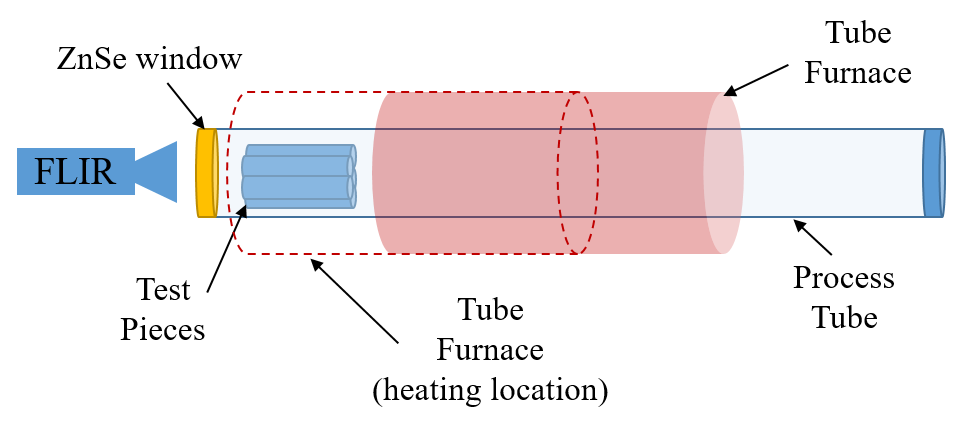
\includegraphics[height=1.75in]{Diagram} 
\par\end{centering}
\caption{Schematic of the experimental setup\label{fig:Furnace-Diagram}}

\vspace{1.75mm}
 
\end{figure}

Conduction cool down experiments were performed on two different assemblies
of graphite cylinders. The cylindrical geometry enabled the temperature
data obtained from the experiments to be used in conjunction with
lower dimension (i.e., 1-D and 2-D) models. Details of each assembly
are provided in Table \ref{tab:Tested-assemblies}. Each assembly
was tested within a quartz tube featuring an ZnSe window through which
the temperature of each rod could be continuously measured using an
infrared (IR) camera. A diagram of the experimental apparatus --
based on that previously used by Gould et al.\cite{GouldNureth,GouldDiss}
-- is shown in Figure \ref{fig:Furnace-Diagram}. Once the assembly
was placed inside the process tube, the process tube was sealed, evacuated
to a rough vacuum, and an electric furnace surrounding the portion
of the tube with the graphite rods was turned on. The assembly was
heated until all rods reached the desired steady state temperature.

\begin{figure}
\begin{centering}
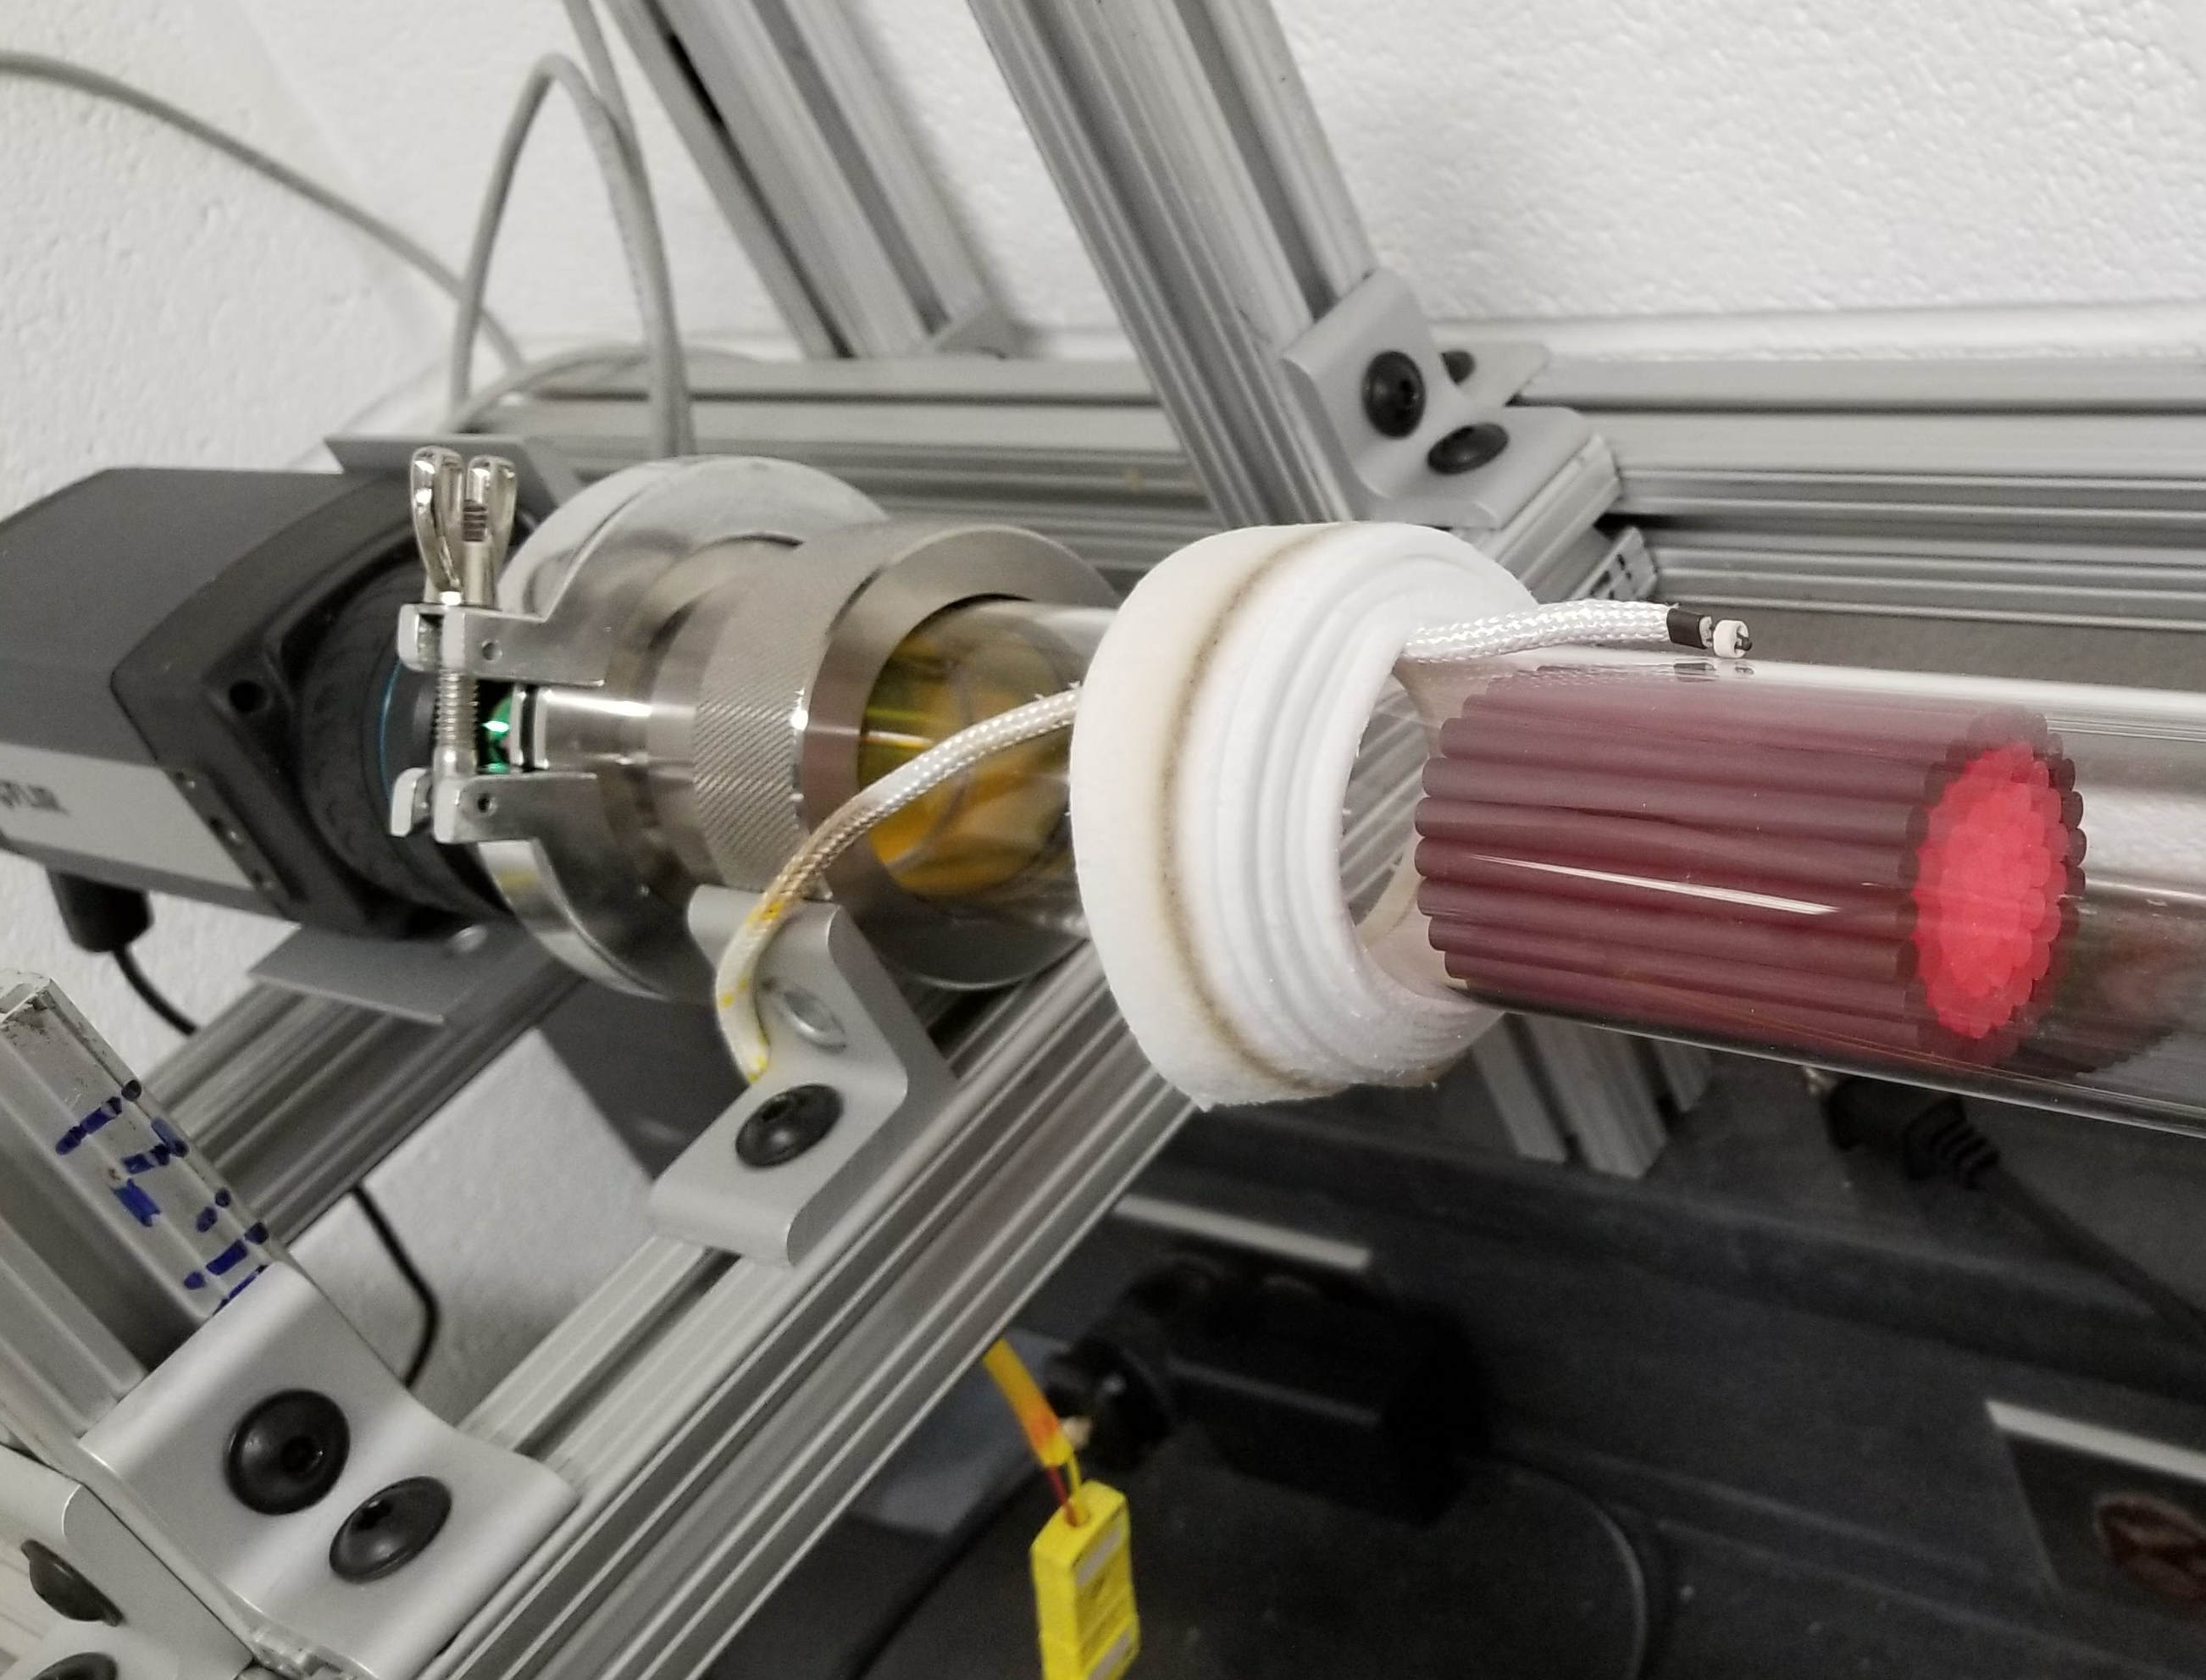
\includegraphics[height=2.75in]{HotRods}\caption{Test assembly beginning to cool. \label{fig:HotRods}}
\par\end{centering}
\vspace{1.75mm}
 
\end{figure}

To initiate the cooling experiment, the radiative heater was switched
off and quickly moved away from its original location surrounding
the assembly. Figure \ref{fig:HotRods} shows a cooling assembly of
graphite rods. Once the heater is removed from its initial position
surrounding the assembly, the temperature of the graphite rods begins
to drop as the heat being conducted out of and radiated away from
the assembly is no longer balanced by the energy input from the furnace.
An IR camera was used to both measure the change in temperature of
each rod as the assembly cooled and provide geometric information
regarding the structure of the assembly. The temperature profiles
observed from these experiments were then used to validate a 2-D combined
DEM/FEM model.

\begin{table}
\begin{centering}
\begin{tabular}{|c|c|}
\hline 
\textbf{\footnotesize{}{}1}{\footnotesize{} } & \textbf{\footnotesize{}{}2}\tabularnewline
\hline 
\begin{minipage}[t]{0.14\textwidth}%
\vspace{0.02in}
 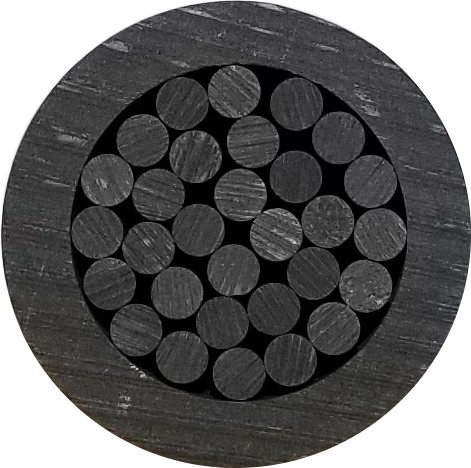
\includegraphics[width=1\linewidth]{GraphiteThinShellPic}\vspace{0.02in}
 %
\end{minipage} & %
\begin{minipage}[t]{0.14\textwidth}%
\vspace{0.02in}
 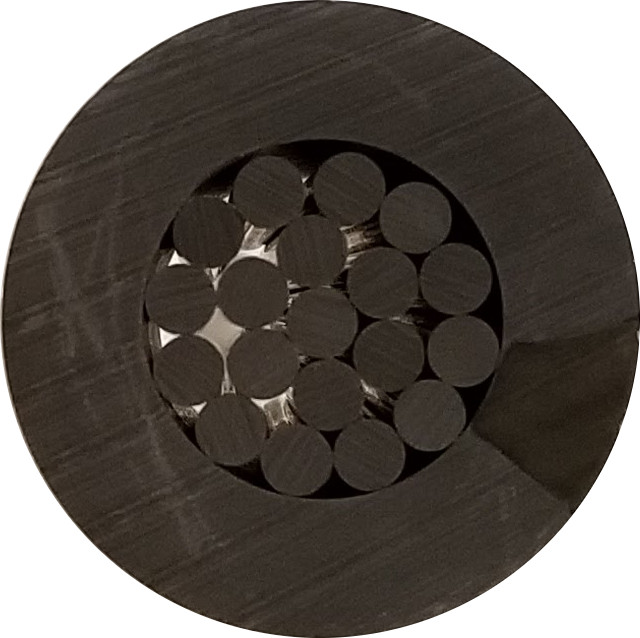
\includegraphics[width=1\linewidth]{ThickShell}\vspace{0.02in}
 %
\end{minipage}\tabularnewline
{\footnotesize{}{}G-348 Graphite}  & {\footnotesize{}{}G-348 Graphite}\tabularnewline
{\footnotesize{}{}30 Rods}  & {\footnotesize{}{}18 Rods}\tabularnewline
{\footnotesize{}{}\SI{2.5}{\milli\meter} Radius }  & {\footnotesize{}{}\SI{2.5}{\milli\meter} Radius }\tabularnewline
{\footnotesize{}{}\SI{72}{\milli\meter} Length}  & {\footnotesize{}{}\SI{72}{\milli\meter} Length}\tabularnewline
{\footnotesize{}{}Thin Shell}  & {\footnotesize{}{}Thick Shell}\tabularnewline
\hline 
\end{tabular}
\par\end{centering}
\centering{}\caption{Details of tested rod assemblies. \label{tab:Tested-assemblies}}
\end{table}

\vspace{-6mm}


\subsection{Discrete Element Method Simulation \label{subsec:N-body-simulation}}

\vspace{-2mm}

Finite element models require very precise geometric information to
accurately simulate the effects of point contacts on inter particle
heat transfer. The geometry of the assembly must be defined with a
sufficient level of precision for a mesh to be created in which nodes
from adjoining rods can be properly connected. Geometry defined using
only the images from the IR camera was found to be insufficiently
accurate for proper mesh connections to be made between adjoining
rods. However, this problem was solved by using an N-body algorithm
to improve the accuracy of the geometry data given from the analysis
of the IR images. This approach not only allowed for a 2--D finite
element model of the rod assembly to be created, but also provided
an opportunity to validate a method an algorithm that could then be
used to create other, more complicated geometries.

Therefore, a 2--D Discrete Element Method (DEM) simulation was used
to modify the rough rod geometry information provided by the IR camera.
For the DEM simulation, each rod is modeled as a 2-D circular particle
in a single plane. The approximate rod centroid locations found from
the IR image analysis were used as initial conditions for the simulation.
Due to the initial rod centroid locations not being precisely accurate,
some rods will initially overlap. These overlapping regions result
in forces -- and thus accelerations -- being applied to the offending
particles. In this 2-D simulation, inter-particle forces are calculated
by modeling any pair of overlapping particles as springs -- with
the repulsion force applied to each particle being a linear function
of their overlap distance. This process is repeated over a large number
of time steps, during which each particle's acceleration and velocity
are tracked, calculated, and integrated to provide new position data
each time step. The newest position data is then again analyzed for
overlaps, following which new forces are applied. This process repeats
until particles are deemed to be moving sufficiently slowly.

In addition to the inter-particle spring forces, two other sources
of force are used in the DEM simulation to constrain the assembly.
First, gravity is accounted for by applying a small, constant force
to each particle in the vertically downward direction. Second, in
the same way that repulsion forces are applied to any particles deemed
to overlap with each other, similar forces are applied to any particle
who's position would have it overlapping with the graphite shell surround
the assembly. These \textquotedblleft wall forces\textquotedblright{}
are applied to the offending particle in the direction normal to the
shell wall at the point of overlap and are again a linear function
of the overlap distance.

Because centroid locations obtained from IR images were used as initial
conditions for this process -- as opposed to random starting locations
-- few overlaps are seen in the initial geometry and the system is
quickly able to converge to a low energy, low velocity state. At this
point, its absolute rod positioning will be almost identical to those
of the actually assembly and the relative rod locations will be sufficiently
accurate to use in a finite elements simulation.

\vspace{-6mm}


\subsection{FEM Model}

\vspace{-2mm}

A commercial multi-physics software, COMSOL, was used to create an
FEM of the experimental assemblies. Due to the very high aspect ratios
of the objects within assemblies, a 2-D model was used \cite{Gould2017c}.
Precise geometry information, i.e. the location of each rod's centroid
in relation to the outer graphite shell, was obtained from the DEM
simulation as discussed in Section \ref{subsec:N-body-simulation}.
This process resulted in the geometry shown in Figure \ref{fig:ComsolMesh}.
The contact locations of adjoining -- as opposed to merely nearby
-- objects in the geometry can be visibly identified in Figure \ref{fig:ComsolMesh}
from the high density regions of the overlain mesh. The inner boundary
of the outer shell is highlighted in blue. Matching the conditions
of the experimental setup, the empty areas surrounding the rods within
the shell were modeled in COMSOL as a vacuum. Thus no material is
seen in between the rods in Figure \ref{fig:ComsolMesh}.

\begin{figure}
\begin{centering}
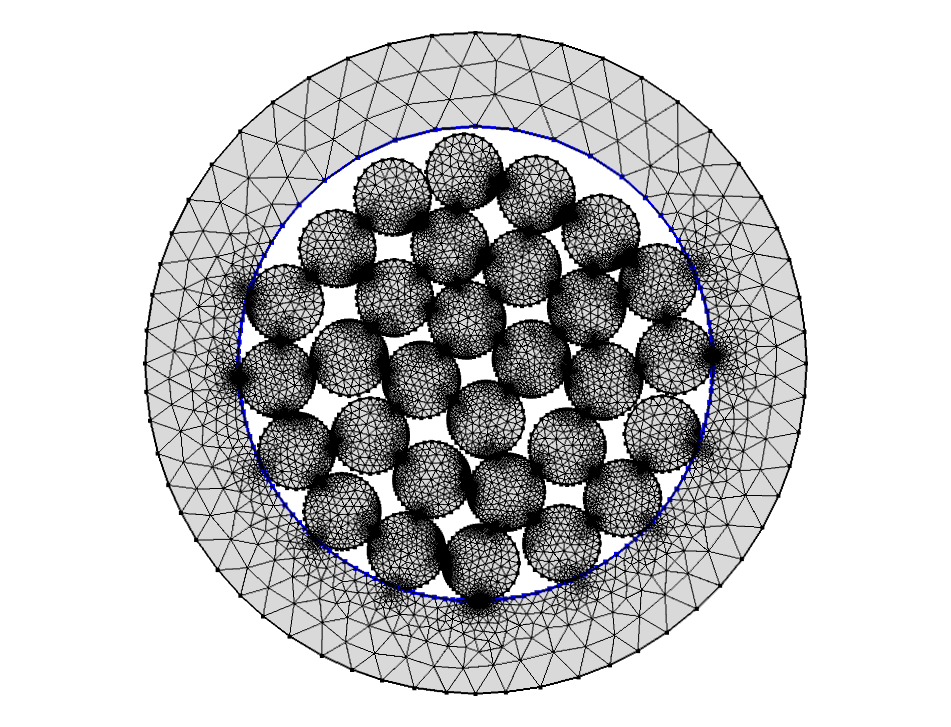
\includegraphics[width=3.25in]{ThinMesh}\caption{Geometry and mesh of thin-shell FEM model. \label{fig:ComsolMesh}}
\par\end{centering}
\vspace{1.75mm}
 
\end{figure}

For the solid domains, heat capacity was defined as a function of
temperature, while a constant value was used for the bulk thermal
conductivity of the material.

The boundary conditions used in the model were surface-to-surface
radiation, thermal contact resistance, and prescribed temperature.
The outer and inner shell boundaries were given time dependent, prescribed
temperature boundary conditions. Specifically, the temperatures of
these boundaries were set to be equal to the median temperature of
the shell face.

Any portion of a rod or shell boundary that was in contact with a
portion of the shell or another rod was subjected to thermal contact
resistance boundary condition. This boundary condition modified the
heat flux passing through the boundary by incorporating a resistance
term at the boundary. A parametric sweep of resistance values was
used to find a near-optimal value of thermal contact resistance for
Assembly 1. This value, \SI{8E-5}{\kelvin\per\watt\per\meter\squared},
was then also used for the COMSOL model of Assembly 2 as well.

Finally, all interior boundaries not in physical contact with another
boundary were set to be gray, diffuse surfaces with emissivity values
of 0.86.

The COMSOL model was a 570 second transient simulation. The model
start time, $t_{0}$, was defined as the moment when, following the
removal of the surrounding tube furnace, the median shell temperature
fell below the lowest measured rod face temperature.

Initial temperatures of the shell and rod faces were obtained from
the IR camera measurements at the time $t_{0}$ and input into the
COMSOL model as a spatial interpolation function. As the simulation
marches through time from $t_{0}$, the thermal energy initially stored
within the rods is diffused and radiated outwards towards the to the
shell, which, due to its lower, prescribed temperature, acts as a
sink.

\vspace{-5.5mm}


\subsection{2-D Results }

\vspace{-2mm}

\begin{figure}[h]
\begin{minipage}[t]{0.45\textwidth}%
\subfloat[Thin shell \label{fig:ThinComsolTemps}]{\centering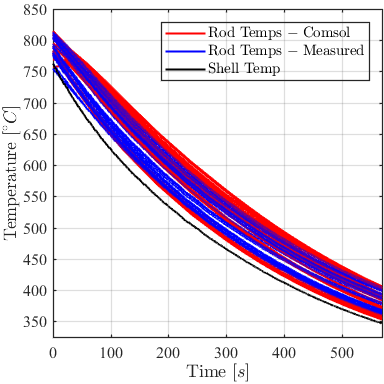
\includegraphics[clip,width=1\columnwidth]{ComsolTempsThin}

}%
\end{minipage}\hfill{}%
\begin{minipage}[t]{0.45\textwidth}%
\subfloat[Thick shell \label{fig:ThickComsolTemps}]{\centering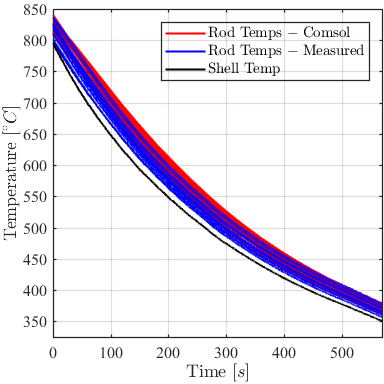
\includegraphics[clip,width=1\linewidth]{ComsolTempsThick}

}%
\end{minipage}\caption{Comparison of measured vs. FEM generated temperatures. \label{fig:ComsolTemps}}

\vspace{1.75mm}
 
\end{figure}

A comparison between the the measured rod temperatures for Assemblies
1 and 2 and the temperatures given by the COMSOL finite element model
is plotted in Figures \ref{fig:ThinComsolTemps} and \ref{fig:ThickComsolTemps},
respectively. The plotted shell temperature is the average temperature
of the graphite shell surrounding each rod and was also the temperature
boundary condition applied to the blue boundary shown in Figure \ref{fig:ComsolMesh}.
The FEM model predicted the temperatures of both assemblies with a
mean error of less than 3 percent in each case.

\vspace{-5mm}


\section{3-D Packed Bed and Comparison to 1-D Model\vspace{-2mm}
 }

\subsection{3-D Discrete Elements Method }

\vspace{-1.75mm}

The discrete elements method is widely used for generating packed
bed geometries \cite{VanAntwerpen2010,VanAntwerpen2012} and was used
here to create the geometry for the 3--D numerical heat transfer
simulation. Although the method cannot easily produce periodic geometries
and is not as precise as some overlap removal methods \cite{Zinchenko1994},
it is far more computationally efficient and thus can be used to create
far larger beds. To create the packed bed geometry that would be used
by the 3--D FEM package, a discrete elements method code was written
in MATLAB to determine 500 fuel-pebble centroid locations that would
form a stable packing structure within a \SI{240}{\milli\meter}
radius cylinder.

Although a custom Matlab DEM code was used in this work, several commercial
DEM packages do exist and would allow for much larger simulations
to be made. However, while powerful, these codes tend to also be both
very complex and expensive. Such power was not needed in this study
as the study focus was on the near wall region of the packed bed and
thus only a low number of particles needed to be modeled. It was decided
that, due to the limited aims of the present study, simply modifying
the previously used 2-D Matlab code would be the most efficient option.
An additional benefit of this decision is that the geometry generated
by the Matlab DEM code could theoretically be used with any available
FEM package.

\begin{figure}[h]
\centering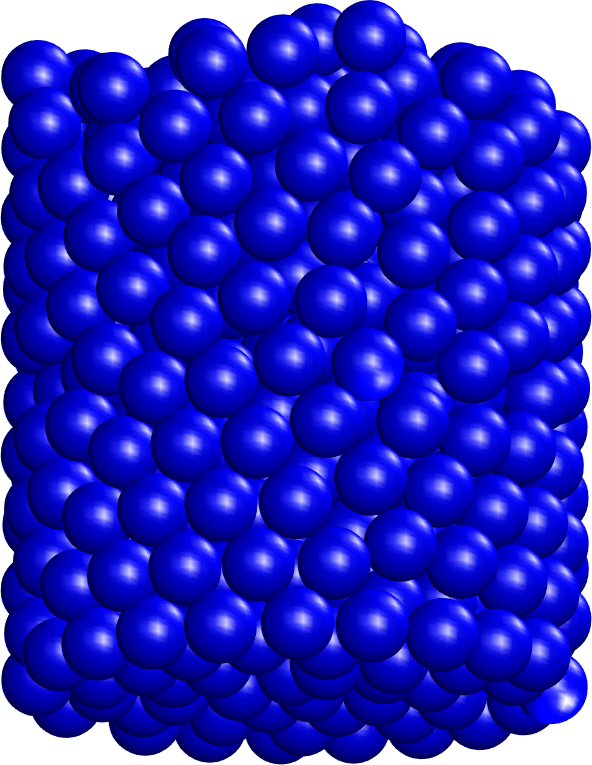
\includegraphics[height=3.5in]{BluePackedBed3}\caption{Packed bed of 500, 60 mm diameter spheres. \label{fig:PackedBed}}

\vspace{1.75mm}
 
\end{figure}

Although based on the code used in Section \ref{subsec:N-body-simulation},
several improvements were made to the code in two different areas.
First, although MATLAB provided a very simple and straightforward
environment for the creation and visualization of a simple DEM code,
its (relatively speaking) slow speed required that several performance
optimizations be applied to the previous code to enable the computation
of a larger number of particles in a higher dimensional space with
reasonable computation times. These improvements included the vectorization
of computations within each time step, using integer and single precision
data types where appropriate, and using initial conditions that slowly
added more particles to the system over time.

This last improvement ended up being the most beneficial. For the
3-D code, the simulation began with each particle being ``dropped''
into the container from random locations rather than prescribing random
initial locations for each particle throughout the container's volume.
By slowly adding each particle to the system over time the code is
able to avoid having to perform calculations on the entire assembly
while the particles are in a high energy state and smaller time steps
are required.

The second major area of improvement to the 2-D code was the use of
Lenard Jones potentials rather than linear spring forces to compute
particle-particle interactions. Using the exponential potentials resulted
in both a greater accuracy and precision in the calculation of each
particle's location, and a decrease in the number of time steps required
to resolve severely overlapping particles. The target overlap distance
-- i.e., the arithmetic difference between the displacement of two
particle centroids and the particle's diameter -- was \SI{0.35}{\milli\meter}.
The simulation was able to achieve a mean overlap distance of \SI{0.3976}{\milli\meter}
with a standard deviation of \SI{0.229}{\milli\meter}. The
finalized geometry produced by the DEM code is shown in Figure \ref{fig:PackedBed}.

\vspace{-6mm}


\subsection{Bed Porosity \label{subsec:Porosity}}

\vspace{-2mm}

\begin{figure}[h]
\begin{minipage}[t]{0.45\textwidth}%
\subfloat[Relative porosity of 500 sphere geometry; calculated using 500 thousand
rays. \label{fig:RelativePorosityPlot}]{\centering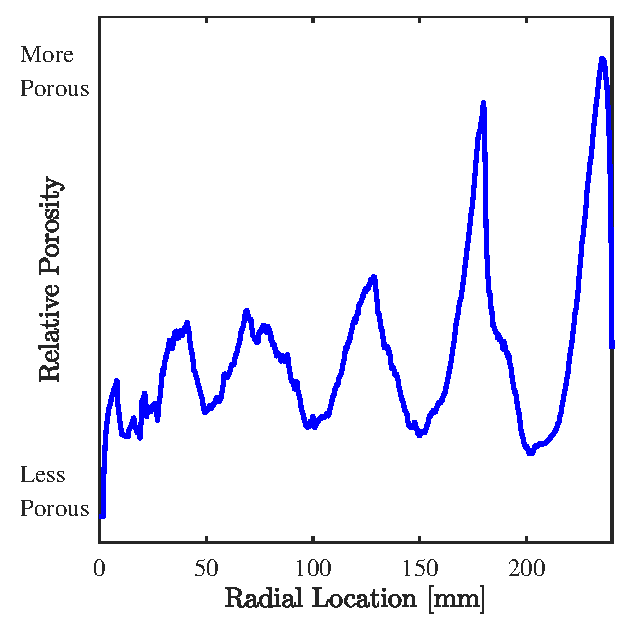
\includegraphics[clip,width=1\linewidth]{RelativePorosity}

}%
\end{minipage}\hfill{}%
\begin{minipage}[t]{0.45\textwidth}%
\subfloat[Graphical depictions of example rays for relative porosity calculation.
\label{fig:SpheresLinesPoros}]{\centering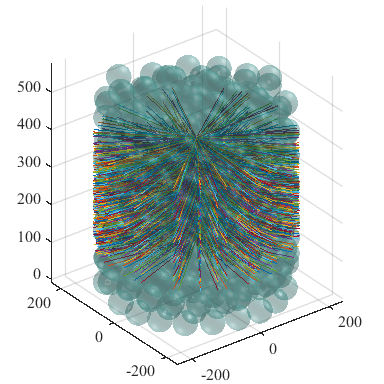
\includegraphics[clip,width=1\linewidth]{LineSphereFig}

}%
\end{minipage}\caption{Relative porosity of packed bed \label{fig:RelPorosity}}

\vspace{1.75mm}
 
\end{figure}

Overall, the DEM generated packed bed possessed an average porosity
of 39\%, matching the values achieved by both Pavlidis and Lathouwers
\cite{Pavlidis2013} using the overlap removal method and Du Toit
\cite{DuToit2008} using a DEM method. This average value was obtained
from calculations performed over the middle 80\% of the bed's length,
where the effects of the top and bottom of the packed bed were minimal.

The relative porosity function plotted in Figure \ref{fig:RelativePorosityPlot}
was computed using a Monte Carlo method. A large number of rays running
radially outward from the center of the packed bed were defined. Examples
of such test rays can be seen in Figure \ref{fig:SpheresLinesPoros}.
A set of radial locations along each ray was tested to determine whether
or not the individual locations were located within the domain of
a solid particle. The tallies for each ray were then recorded as a
function of the radial location of each test point. As shown in Figure
\ref{fig:RelativePorosityPlot}, the relative porosity of the bed
continues to oscillate all the way through the bed center. This continued
oscillation confirms that the entire packed bed can be considered
in the ``near-wall'' region. Because of this, many previously developed
empirical correlations for packed beds are not valid for this particular
geometry.

\vspace{-6mm}


\subsection{Geometry and Boundary Conditions}

\vspace{-2mm}

\begin{table}
\begin{centering}
\caption{Geometric parameters of individual particles and packed bed. \label{tab:GeometricParameters}}
\par\end{centering}
\centering{}%
\begin{tabular}{|c|r@{\extracolsep{0pt}.}l|}
\hline 
\textbf{Sphere Radius} & \multicolumn{2}{c|}{\SI{25}{\milli\meter}}\tabularnewline
\hline 
\textbf{Shell Thickness} & \multicolumn{2}{c|}{\SI{5}{\milli\meter}}\tabularnewline
\hline 
\textbf{Number of Particles} & \multicolumn{2}{c|}{500}\tabularnewline
\hline 
\textbf{Bed Radius} & \multicolumn{2}{c|}{\SI{240}{\milli\meter}}\tabularnewline
\hline 
\textbf{Bed Height} & \multicolumn{2}{c|}{\SI{582}{\milli\meter}}\tabularnewline
\hline 
\textbf{Mean Contact Area} & \multicolumn{2}{c|}{\SI{28.2}{\milli\meter\squared}}\tabularnewline
\hline 
\end{tabular}
\end{table}

Each spherical particle was modeled as a \SI{25}{\milli\meter}
radius sphere surrounded by a \SI{5}{\milli\meter} thick shell.
These dimensions match those of the fuel particles produced by the
NUKEM company for the Thorium High-Temperature Reactor. The splitting
of the fuel pebbles into the two separate domains was required as
only the inner \SI{25}{\milli\meter} regions (the `Spheres'
domains) of the NUKEM fuel pebbles contained fissile material; the
outer \SI{5}{\milli\meter} layer of each pebble (the `Spherical
Shells' domains) was made of graphite alone.

These shapes were created in the SOLIDWORKS CAD program and placed
in an assembly at the centroid locations previously determined by
the DEM model. This geometry was then exported into the ANSYS Design
Modeler program for final processing. Using the Design Modeler software,
two additional domains (in addition to the `Spherical Shells' and
`Spheres' domains imported from the CAD software) were created using
Boolean operations. Additionally, the overlapping areas within the
`Spherical Shells' domain were sliced as to implement the ``capped''
method described by Ferng and Lin \cite{Ferng2014}.

\begin{figure}
\begin{minipage}[t]{0.4\textwidth}%
\begin{center}
\subfloat[Spheres \label{fig:GreenSpheres}]{\centering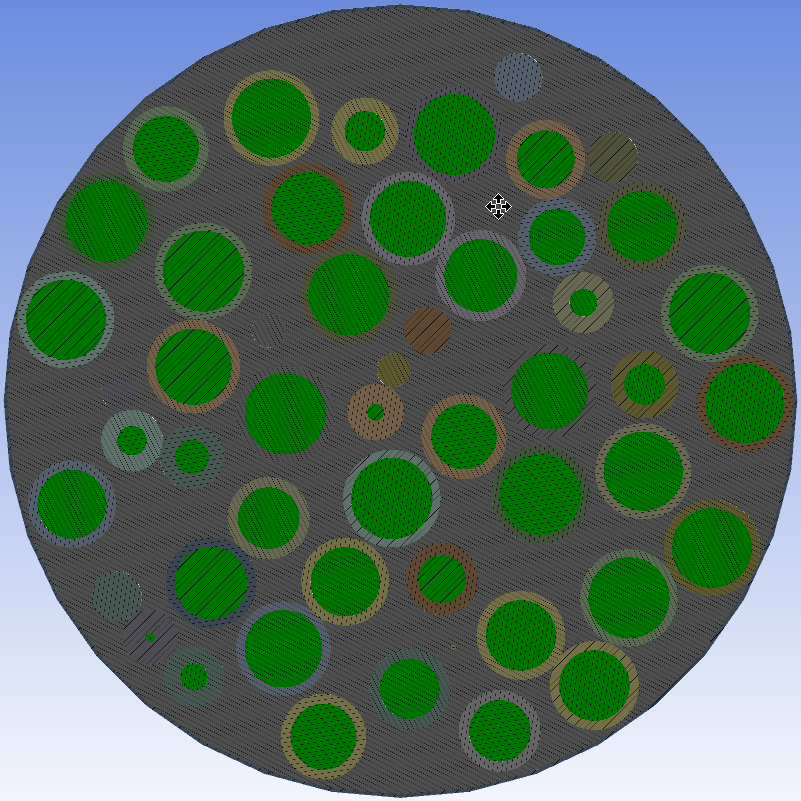
\includegraphics[clip,width=1\linewidth]{GreenSpheres}

}
\par\end{center}%
\end{minipage}\hfill{}%
\begin{minipage}[t]{0.4\textwidth}%
\begin{center}
\subfloat[Spherical Shells \label{fig:GreenShells}]{\centering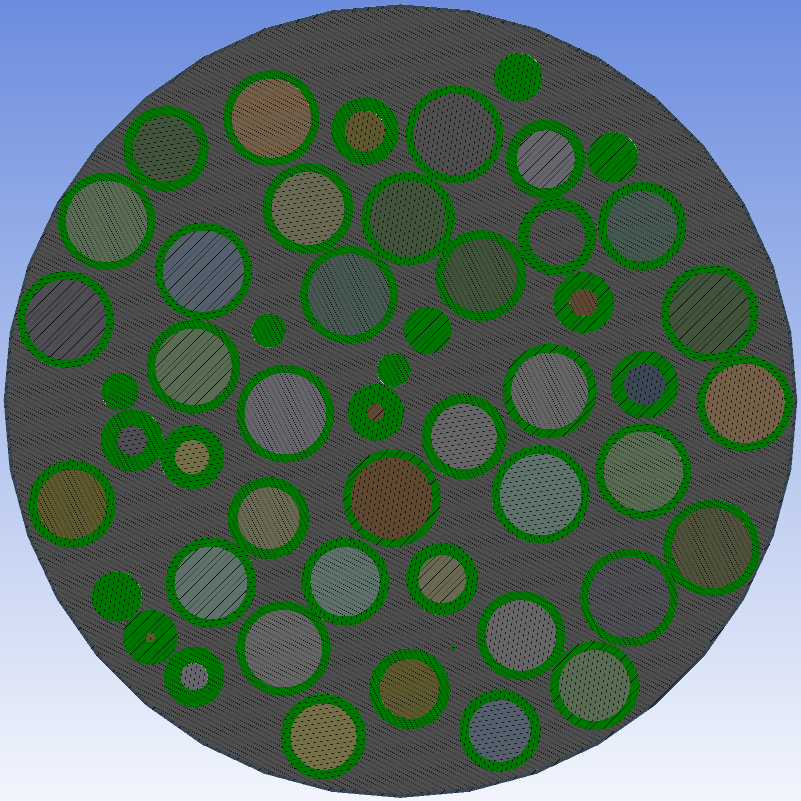
\includegraphics[clip,width=1\linewidth]{GreenShells}

}
\par\end{center}%
\end{minipage}\bigskip{}

\begin{minipage}[t]{0.4\textwidth}%
\begin{center}
\subfloat[Solid Air \label{fig:GreenAir}]{\centering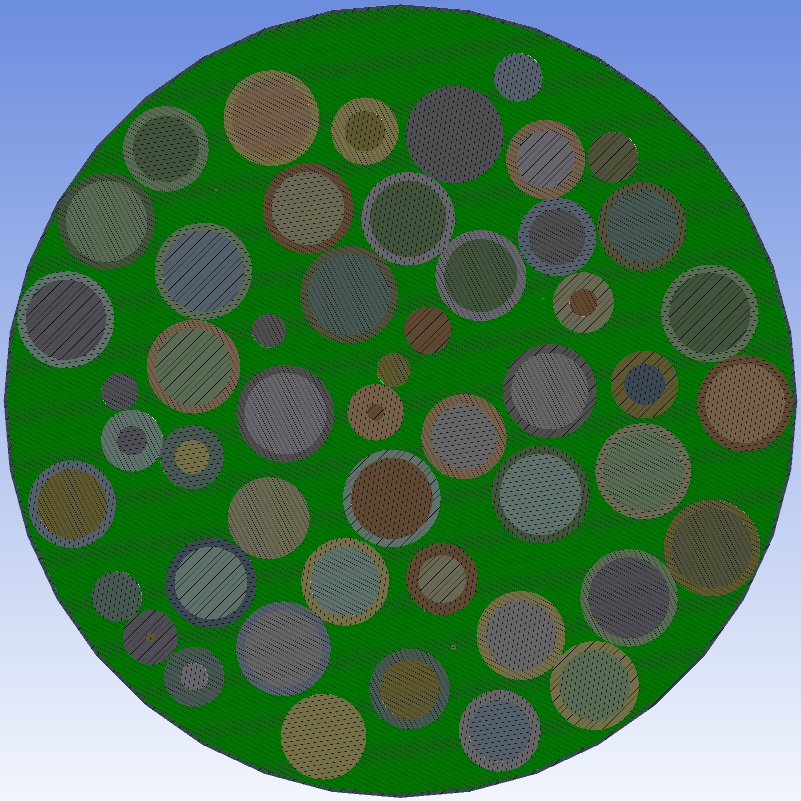
\includegraphics[clip,width=1\linewidth]{GreenAir}

}
\par\end{center}%
\end{minipage}\hfill{}%
\begin{minipage}[t]{0.4\textwidth}%
\begin{center}
\subfloat[Cylindrical Shell \label{fig:GreenCylinder}]{\centering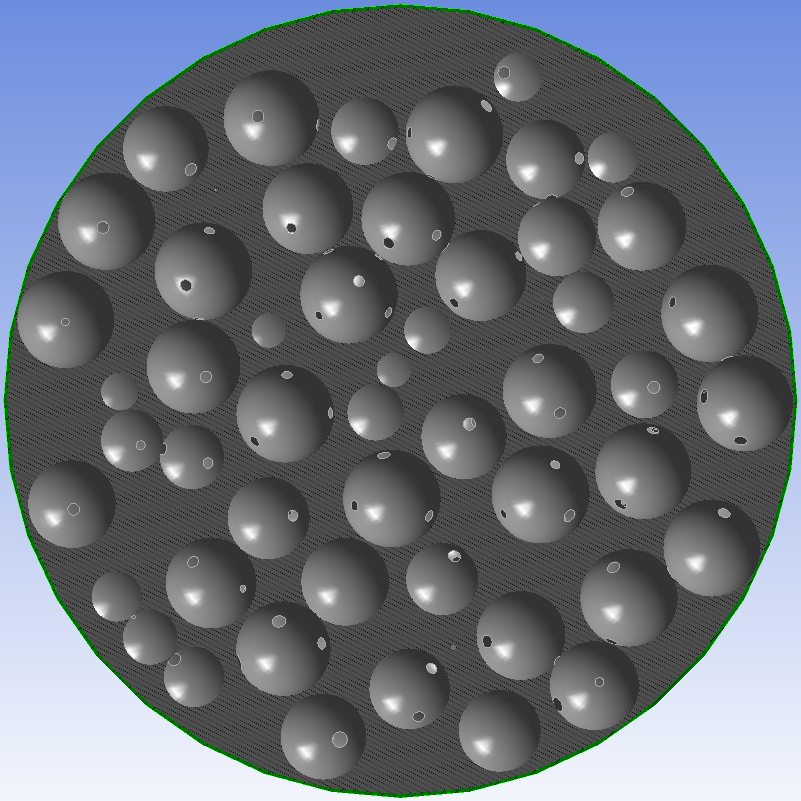
\includegraphics[clip,width=1\linewidth]{GreenCylinder2}

}
\par\end{center}%
\end{minipage}\caption{Cross section of meshed geometry with individual domains identified
in green. \label{fig:4Domains}}

\vspace{1.75mm}
 
\end{figure}

A domain referred to as the `Solid Air' region was created in the
volume between the particles within the packed bed and was defined
to be a solid domain possessing the material properties of air. As
buoyancy forces, fluid flow, and radiative heat transfer are not considered
by this model, modeling this region as a solid material was acceptable.

Surrounding the air, sphere, and shell domains is the `Cylindrical
Shell' domain. This domain is a \SI{2.5}{\milli\meter} thick
cylindrical shell. A cross section of this shell is shown highlighted
in green in Figure \ref{fig:GreenCylinder}. The top and bottom faces
of the cylindrical shell -- i.e. the domain's exterior faces that
are parallel to the cross section shown in Figure \ref{fig:GreenCylinder}
-- were defined as insulated surfaces while a constant temperature
boundary condition of \SI{300}{\kelvin} was applied to the outermost
wall of the cylindrical shell.

Perfect thermal contact was assumed to exist between the Spherical
Shell domains and the Sphere domains, as well as between the Solid
Air domain and the Cylindrical Shell domains. The thermal contacts
between individual shells were not assumed to be perfect. Rather,
the thermal contact conductance between individual fuel particles
was input as a function of their surface roughness. Finally, the bottom
and top faces of both the Solid Air and Cylindrical Shell domains
were defined to be insulated surfaces.

To represent the decay heat generated within each particle following
an air-ingress accident, a time-dependent generation function was
applied to each of the `Spheres' domains. The time-dependent decay
heat generation rate reported by Teuchert et. al for pebble bed reactors
as a function of steady state power was used \cite{Teuchert1992}.
For the NUKEM pebbles, the average total generation rate for each
pebble under steady state conditions was specified to be \SI{1.4}{\kilo\watt}
under steady state operation \cite{PebblesThermalConductivity}.

\vspace{-6mm}


\subsection{1--D Model}

\vspace{-2mm}

\begin{table}
\caption{1--D homogeneous model data \label{tab:PackedHomoModelData}}

\centering{}%
\begin{tabular}{|c|c|c|c|}
\hline 
 & \multicolumn{1}{c|}{\textbf{(1)}} & \textbf{(2)}  & \textbf{(3)}\tabularnewline
\hline 
 & \textbf{Unoxidized,}  & \textbf{Unoxidized,}  & \textbf{Oxidized and }\tabularnewline
 & \textbf{ Perfect Contact {[}}\ref{fig:PerfectOptimal}\textbf{{]}}  & \textbf{Contact Resistance {[}}\ref{fig:VirginOptimal}\textbf{{]}}  & \textbf{Irradiated {[}}\ref{fig:LowKoptimal}\textbf{{]}}\tabularnewline
\hline 
\textbf{$\boldsymbol{k_{eff}}$$\left[\si[per-mode=fraction]{\watt\per\meter\per\kelvin}\right]$$\vphantom{\sum_{5_{5_{6_{_{\$}}}}}^{5^{5^{\%}}}}$}  & {\small{}{}6.6665}  & {\small{}{}2.5469}  & {\small{}{}2.1744}\tabularnewline
\hline 
\end{tabular}
\end{table}

A 1--D radial model was created to provide a comparison with the
results from the 3--D packed bed model. The system was modeled as
a homogeneous domain with modified material properties. The density
and heat capacity of the representative domain were defined to be
porosity-weighted average of that used for the solid particles in
the 3--D simulation.

For thermal conductivity, an inverse heat transfer method was used
to find the optimal $k_{eff}$ for the packed bed. After computing
the direct solution to the heat equation for 1-D homogeneous model,
an optimization process was performed with the goal of minimizing
the error between both the maximum and mean sphere temperature reported
by the 1--D and 3--D models. The thermal conductivity value found
by the optimization process to minimize this error was defined to
be the $k_{eff}$ of the 1-D model. Results obtained from the 1--D
model using this optimized $k_{eff}$ are also compared to those given
by the value of $k_{eff}$ provided by Teuchert, Haas, and Van Heek
\cite{Teuchert1992} for a pebble bed reactor core.

\vspace{-6mm}


\subsection{3-D Results }

\vspace{-2mm}

\begin{figure}[h]
\begin{minipage}[t]{0.49\textwidth}%
\subfloat[Cross section of bed 0.3 m above bed base. \label{fig:AnsysXY}]{\centering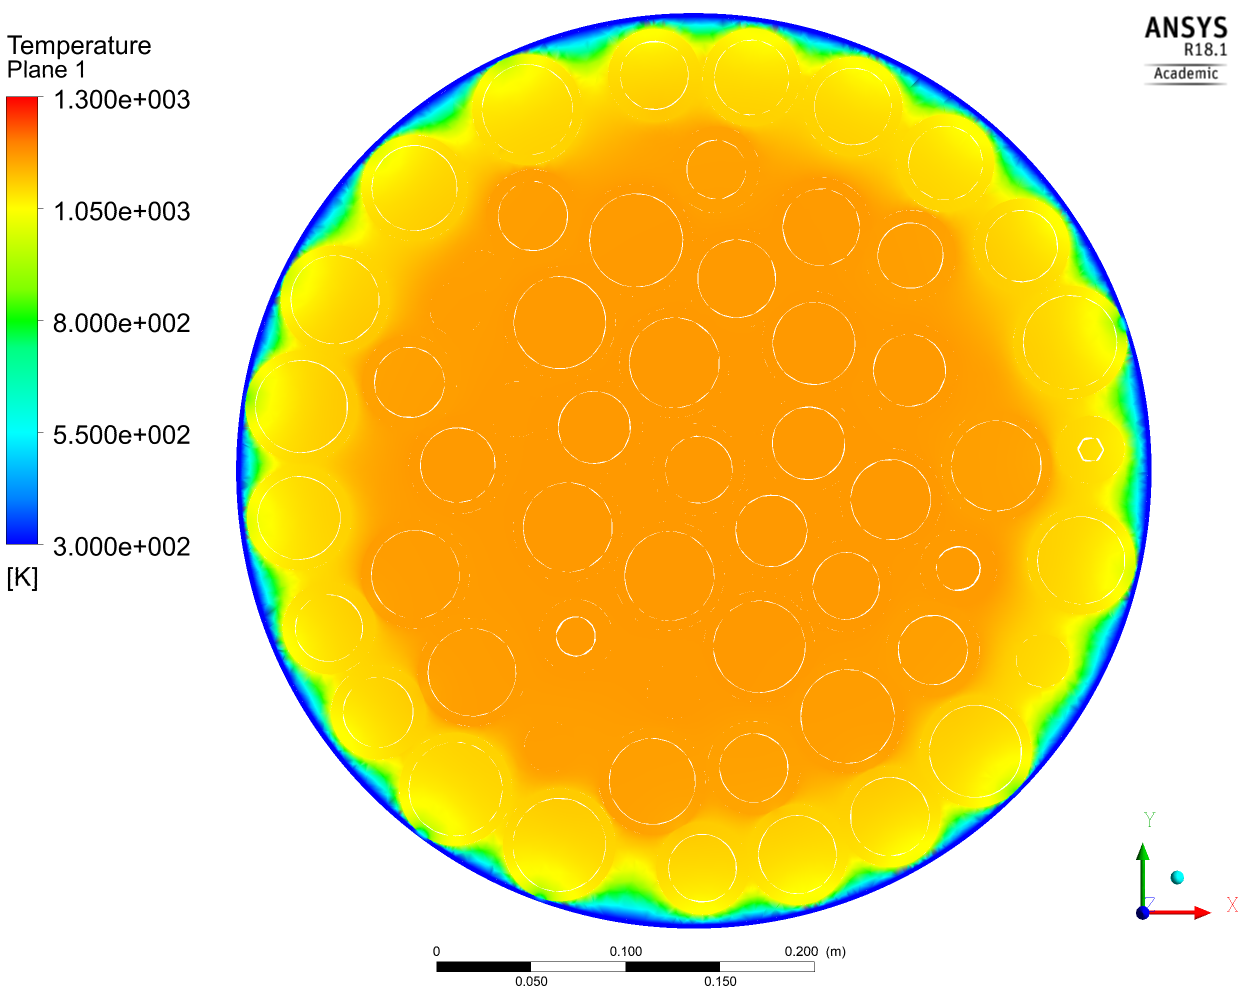
\includegraphics[clip,width=1\linewidth]{NoResistance0-3XY100}

}%
\end{minipage}\hfill{}%
\begin{minipage}[t]{0.49\textwidth}%
\subfloat[Axial slice through mid-plane of packed bed. \label{fig:AnsysZX}]{\centering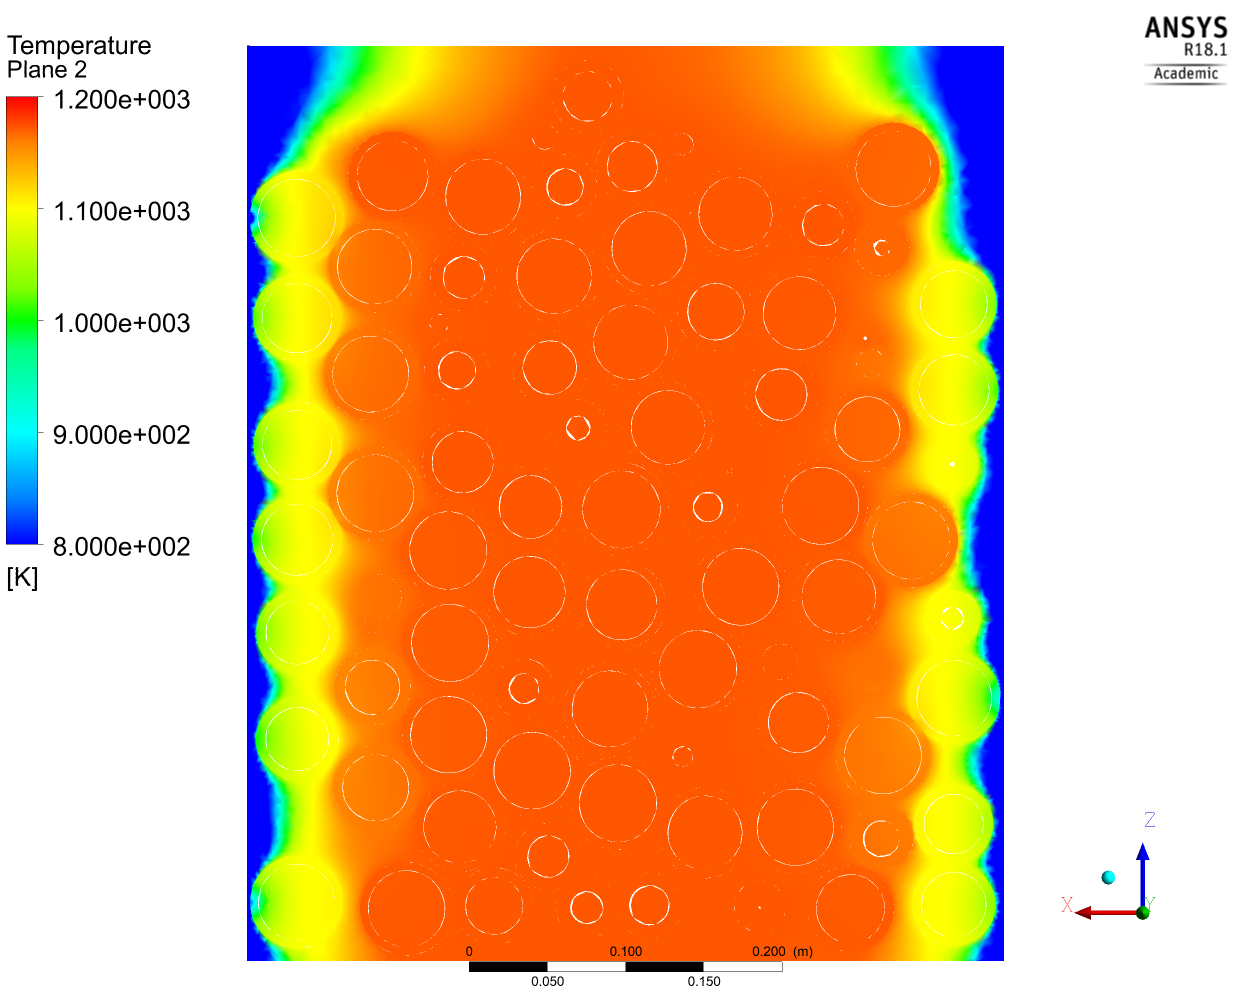
\includegraphics[clip,width=1\linewidth]{NoResistanceZX100}

}%
\end{minipage}\caption{Temperature of unoxidized packed bed with no contact resistance at
100 s. \label{fig:AnsysImages100}}

\vspace{1.75mm}
 
\end{figure}

Data sets from three different simulations were analyzed: unoxidized
graphite spheres in perfect thermal contact with one another (Case
1), unoxidized graphite spheres with contract resistance (Case 2),
and oxidized and irradiated graphite spheres with contact resistance
(Case 3). Case 1 is used as a limiting case example in which the graphite
still possesses its full density and thermal conductivity and in which
any thermal contact resistance between individual spheres is negligible.
In Case 2, the graphite spheres were assumed to have an unoxidized,
smooth surface and the effects of thermal contact resistance were
added to the model. Finally, in Case 3, both the effects of oxidation
and irradiation were included in the analysis. Following irradiation,
the thermal conductivity of the NUKEM particles has previously been
shown to decrease drastically \cite{PebblesThermalConductivity}.
And, as any fuel particles that would be involved in an air ingress
accident are almost certain to have undergone significant irradiation,
for Case 3, in addition to modeling the effects of thermal contact
resistance between individual oxidized fuel spheres, the bulk thermal
conductivity value of the spheres and shells domains was lowered to
the \SI[per-mode=fraction]{30}{\watt\per\meter\per\kelvin}
value reported by Harms and Trauger\cite{PebblesThermalConductivity}.

\begin{figure}[h]
\begin{minipage}[t]{0.45\textwidth}%
\subfloat[Unoxidized graphite in perfect thermal contact. \label{fig:PerfectOptimal}]{\centering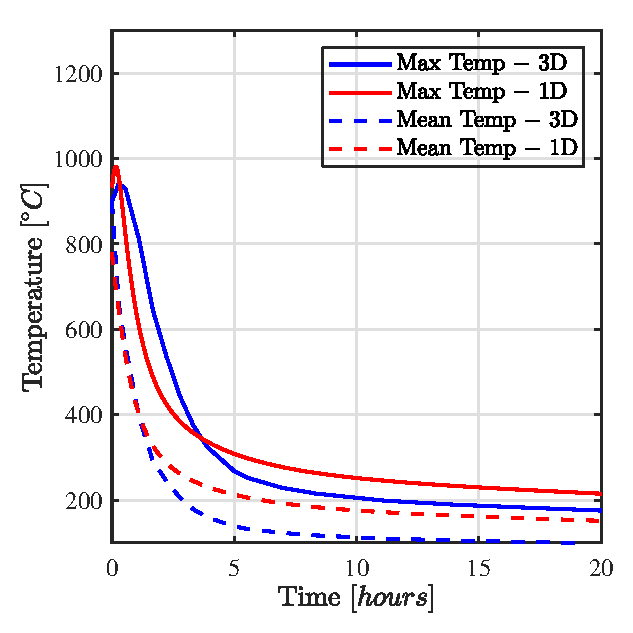
\includegraphics[clip,width=1\linewidth]{PerfectOptimal}

}%
\end{minipage}\hfill{}%
\begin{minipage}[t]{0.45\textwidth}%
\subfloat[Unoxidized graphite with contact resistance. \label{fig:VirginOptimal}]{\centering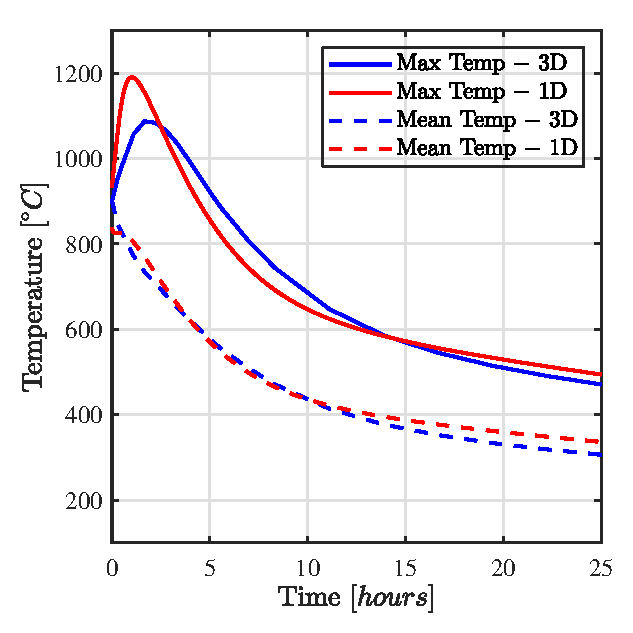
\includegraphics[clip,width=1\linewidth]{VirginOptimal}

}%
\end{minipage}\bigskip{}

\begin{centering}
\begin{minipage}[t]{0.45\textwidth}%
\centering\subfloat[Irradiated and oxidized graphite with contact resistance. \label{fig:LowKoptimal}]{\centering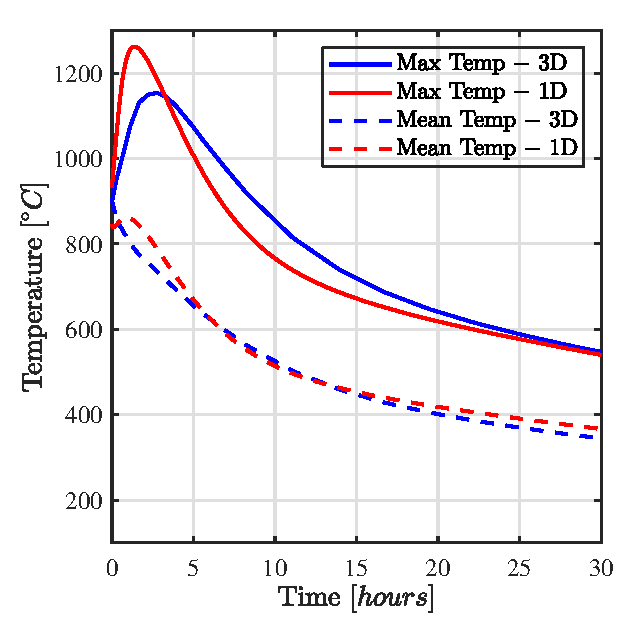
\includegraphics[clip,width=1\linewidth]{LowKoptimal}

}%
\end{minipage}\caption{Plots of bed maximum and mean temperatures over time as determined
by both 3--D CFD and the 1--D homogeneous code with an optimal $k_{eff}$.
\label{fig:OptimalKplots}}
\par\end{centering}
\vspace{1.75mm}
 
\end{figure}

In Figure \ref{fig:AnsysImages100}, pseudo-color temperature plots
of two different planes are shown from the Case 1 CFD model, 100 seconds
into the run. Table \ref{tab:PackedHomoModelData} presents the results
of the effective thermal conductivity optimization algorithm are shown
for each case. In each case, the optimal value of thermal conductivity
to best match the 3--D CFD results was significantly lower than that
previously suggested by Teuchert, Haas, and Van Heek \cite{Teuchert1992}
for an entire pebble bed reactor core. This difference is likely a
result of the packed bed geometry simulated in the 3--D CFD model
not being large enough for wall effects to become negligible.

Figure \ref{fig:OptimalKplots} plots mean and maximum bed temperatures
for each of the three analyzed cases as calculated by both the 3--D
CFD and 1--D homogeneous models. The 1--D code over predicted the
bed maximum temperature by \SI{39}{\kelvin}, \SI{97}{\kelvin},
and \SI{108}{\kelvin} for cases 1, 2, and 3, respectively. It
should be remembered that the 1--D results shown in Figure \ref{fig:OptimalKplots}
represent the accuracy of the best possible 1-D, homogeneous model.
In the real world, the accuracy of any such model is likely to be
far worse.

\vspace{-6mm}


\section{Conclusions}

\vspace{-3.5mm}

Although it is obviously not ideal for full core, large scale simulations,
the MATLAB computational environment proved readily capable of performing
smaller DEM simulations.

By definition, 1-D homogeneous models cannot model the effects of
individual point thermal contacts on heat transfer. At best, in a
sufficiently uniform packed bed in which the aggregate effects of
all point contacts will be both consistent and linear, 1-D homogeneous
models can provide reasonable estimates of bulk heat transfer. However,
previous reported values of effective thermal conductivity for PBR
cores should not be taken as gospel in the near-wall region. Given
the temperature over--predictions seen even when using the best possible
$k_{eff}$ values, any 1--D homogeneous model claiming to accurately
represent the near-wall region of a PBR bed should be viewed skeptically
if precise temperature values are needed in this region. At the very
least, any attempt to produce such a model should take into account
the both the irradiation and oxidation history of the graphite fuel
particles under consideration.

\FloatBarrier

\section*{Acknowledgments}

This material is based upon work supported by the Department of Energy
under Awards DE-NE0008412.

The author would like to thank Mark Shattuck for providing the initial
code upon which the DEM code used here was built.

 \bibliographystyle{ans}
\bibliography{Packing,SVRbib,GouldBibtex}

\end{document}
